\section{Our Approach} % (fold)
\label{sec:approach}

A typical phishing scenario starts with a fraudster sending an email to a potential victim. The end goal is to lure the user into clicking on a link to provide critical information regarding their banking details (e.g., online banking credentials, account number, identification details). Figure~\ref{fig:phishing-email} depicts a template of such an email.

\begin{figure}[hp!]
  \begin{center}
    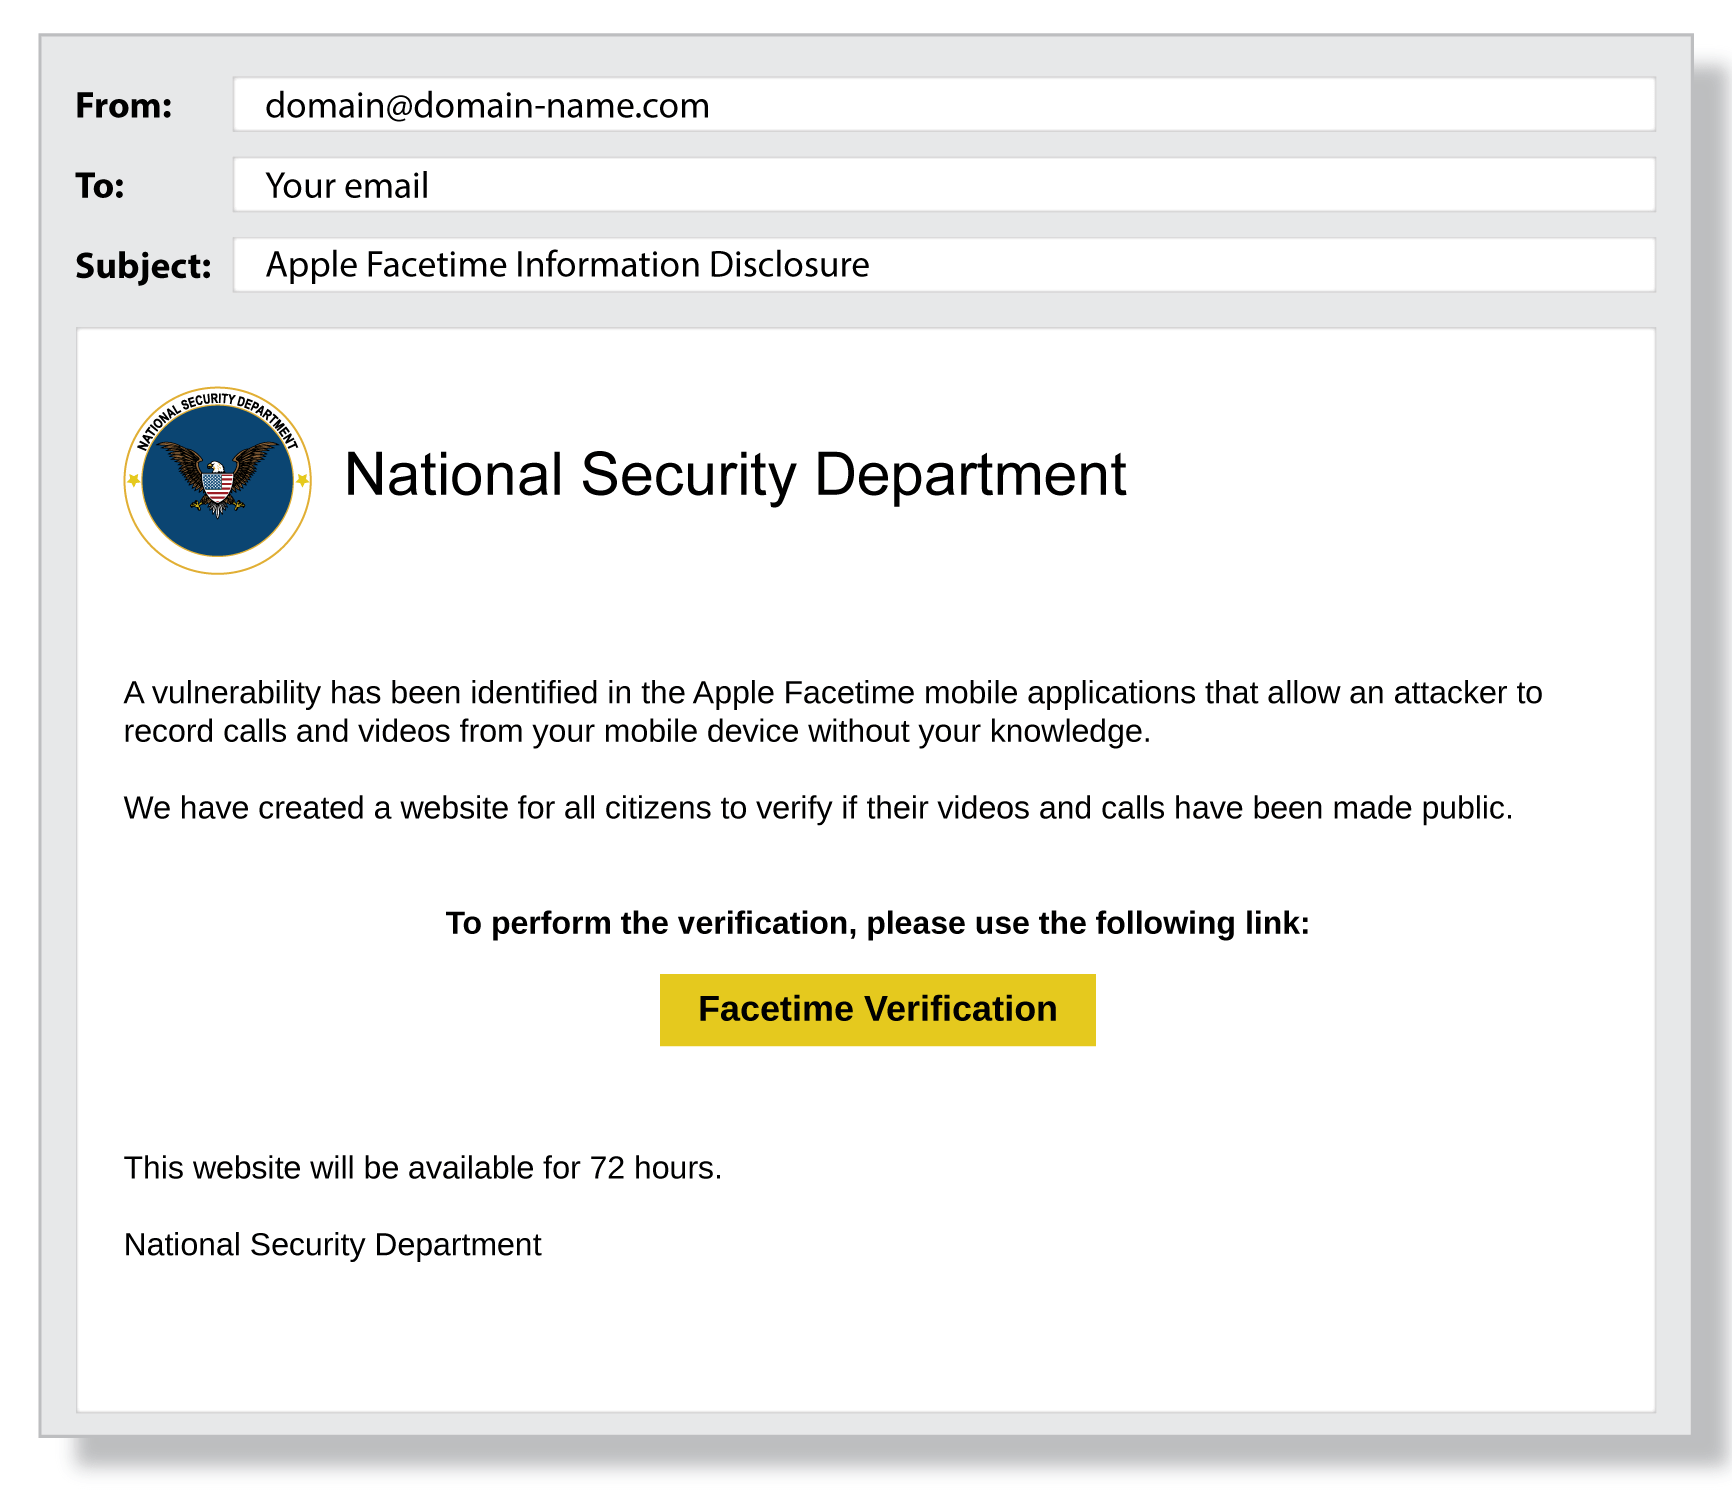
\includegraphics[width=0.85\textwidth]{phishing-email-eg}
  \end{center}
  \caption{Example of Phishing Email}\label{fig:phishing-email}
\end{figure}

We use a \gls{nlp}-based \emph{text analysis}\footnote{The text analysis algorithm is out of the scope of this paper.}  technique to understand the email and select the link(s). We strip each link of the protocol (e.g., HTTP, HTTPS) and query parameters and extract the \emph{domain name}. Next we analyse the domain name and look for similar phonetically-sounding domain names. Finally, we scrutinise the web forms corresponding to the identified domain names and assess their closeness. We discuss both techniques in this section.

\subsection{Link Analysis} % (fold)
\label{sub:approach-link-analysis}

We define a \emph{string} as a finite sequence of characters over an alphabet. We argue that two strings $\mathsf{s_1}$ and $\mathsf{s_2}$ are strings sharing some closeness in their representation. Definition~\ref{theo:phonetic-names} defines phonetic similarity in our context.  

\begin{definition}[Phonetically Similar Strings]
  \label{theo:phonetic-names}
  Given a string $\mathsf{S}$, a string $\mathsf{S^\prime}$ sounds phonetically similar to $\mathsf{S}$ if  $\mathsf{S^\prime}$ is a \emph{sub-string} of $\mathsf{S}$ starting from the same character, or $\mathsf{S^\prime}$ is a \emph{super-string} of $\mathsf{S}$.  
\end{definition}

For example, given the string {\texttt{standardbank}}, {\texttt{standardbank1}} is phonetically similar as a super-string; {\texttt{standarbank}} is also phonetically similar as a sub-string with an inexact match. We execute the the match operation (both exact and inexact) using  a \emph{trie}~\cite{leis-kemper-neumann:2013,morrison:1968,gusfield:1997,ukkonen:1995} data structure. A trie (or suffix tree) is a \emph{hierarchical} data structure used to efficiently represent a string and its suffixes.

We expand the English alphabet with digits (alphanumeric) and a specical character admitted in domain names. Let $\Sigma$ represent our new alphabet; $\Sigma = \{a, b, \ldots, z\}~\bigcup~\{0, 1, \ldots, 9\}~\bigcup~\{-\}$. We construct the suffix tree following Ukkonen's algorithm~\cite{ukkonen:1995}. The construction algorithm starts with a root node. For each distinct character in the string, a new edge is added. The edges are sometimes combined (or compressed) to avoid longer paths. 


Once the trie is constructed, we can execute an \emph{exact} match search of substrings stating with the first characted in the domain name.  This operation is performed by visiting the trie from the root all the way down to the leaves and identifying the valid substrings. In parallel, we perform an \emph{inexact} match search for substrings starting from the initial character. The inexact search tolerates mismatches during the search.  

On the other hand, we construct the super-strings that are phonetically close to the domain name by augmenting the name with a character, a digit or a specical character in the alphabet. Definition~\ref{theo:super-strs} clarifies the relationship between a string and a super-string. Note that the new character can be inserted anywhere in the initial name. 

\begin{definition}[Super Strings]
  \label{theo:super-strs}
  Given a string $\mathsf{Nm}$, a super-string of $\mathsf{Nm}$ is a string whose suffixes include $\mathsf{Nm}$.
\end{definition}

The extraction of the substrings and super-strings of a given domain name is summarised in Algorithm~\ref{alg:la-name-extraction}. It takes the initial domain as input and returns a set of phonetically related names. The function $\mathit{construct\_trie}()$ generates the suffix tree using the initial domain name. Then, from the beginning of the domain name, we extract sub parts and check if they represent a valid substring using both the exact ($\mathit{exact\_match}$) and inexact ($\mathit{inexact\_match}$) matches (lines $3 -- 6$). Finally we generate the super-strings and add them to the list of potential domain names (line $7$). Note that during the inexact match as well as the super-string, characters that visually look like the ones in the initial alphabet are also included. (give the example of a cyrillic character between a and ...)

\SetKwInput{KwInput}{Input}
\SetKwInput{KwOutput}{Output}

\begin{algorithm}[pht!]
    \DontPrintSemicolon
    \KwInput{$\mathsf{N}$ \atcp{Initial domain name}}
    \KwOutput{$\mathrm{S}$ \atcp{Phonetically related names}}

    $\mathsf{T} \gets \mathit{construct\_trie}(\mathsf{N})$\;

    $\mathrm{S} \gets \{\}$\;

    \For{$\mathsf{pos}=1,\ldots ,|\mathsf{N}|$}{
      $\mathsf{cur\_str} \gets \mathit{extract\_string}(1, \mathsf{pos}, \mathsf{N})$\;
      \If{$\mathit{exact\_match}(\mathsf{cur\_str}, \mathsf{T}, \mathsf{N}) \vee \mathit{inexact\_match}(\mathsf{cur\_str}, \mathsf{T}, \mathsf{N})$}{
        $\mathrm{S} \gets \mathrm{S} ~\bigcup~ \{\mathsf{cur\_str}\}$\;
      }
    }
    
    $\mathrm{S}\gets\mathit{add\_supers}(\mathsf{N}, \mathrm{S})$\;

    $\KwRet~~\mathsf{S}$\;

    \SetKwProg{fn}{Function}{}{}
    \SetKwFunction{initatenegofunc}{$\mathit{initiate\_negotiation}$}{}
    \SetKwFunction{handlemsgfunc}{$\mathit{handle\_message}$}{}
    \;

\caption{Link Analysis}
\label{alg:la-name-extraction}
\end{algorithm}

Discuss an illustration of the algorithm...

Each new domain name obtained from Algorithm~\ref{alg:la-name-extraction} is then extended with a potential domain extension (e.g., {\texttt{.com}}, {\texttt{.net}}, {\texttt{.org}}, {\texttt{.xyz}}, etc.). The resulting string is used to query to domain database about their validity. We propose an adaptaion of the \emph{Map-Reduce} algorithm~\cite{dean-dhemawhat:2008} to handle this process. The \emph{Mapper} takes a key and a pair of strings, a potential domain name and an extension. It concatenates the strings and queries the domain database about the validity of the newly constructed domain using {\texttt{nslookup}}\footnote{The documentation about the nslookup command can be found at \url{https://linux.die.net/man/1/nslookup}}. The mapper returns a $0$ or a $1$ indicating whether the domain is valid or not. As for the \emph{Reducer}, it compiles the intermediate results and only retains the constructed strings that prove to be a valid domain name. The web pages behind the domain names validated by the Map-Reduce algorithm are further  analysed. We discuss this in Section~\ref{sub:approach-web-page-analysis}.

Maybe add a graphical representation of the protocol...
Provide an illustration... Ensure that all illustrations are related...

% subsection Link Analysis (end)

\subsection{Web Page Analysis} % (fold)
\label{sub:approach-web-page-analysis}

The second part of our analysis looks for the Web page corresponding to a valid domain name identified in Section~\ref{sub:approach-link-analysis}. We access the HTML source of the page and extract the FORM tag within the page. The form contains a set of components that capture user information. Our goal is to convert the form into a graph and latter build a \gls{gnn} to help classify whether or not a given graph falls within the banking domain. 

To generate the initial graph, we iterate over the children of the HTML form. For each component (e.g., \emph{label}, \emph{input}, \emph{textarea}, etc.), we create a corresponding vertex. The edges between the vertices reflect the sequence in which the components are arranged in the form.  Figure~\ref{fig:form-to-graph-eg} depicts the transformation from an HTML form to a graph. The diagram on the left (Subfigure~\ref{fig:init-form}) represents the form, while the one on the right (Subfigure~\ref{fig:final-form}) represents the resulting graph. We curated Web forms from various websites and created a dataset of graphs. The reader should note that we unify the graph size (especially the number of vertices) by padding the smaller ones.

\begin{figure*}[th!]
    \centering
    \begin{subfigure}[t]{0.5\textwidth}
        \centering
        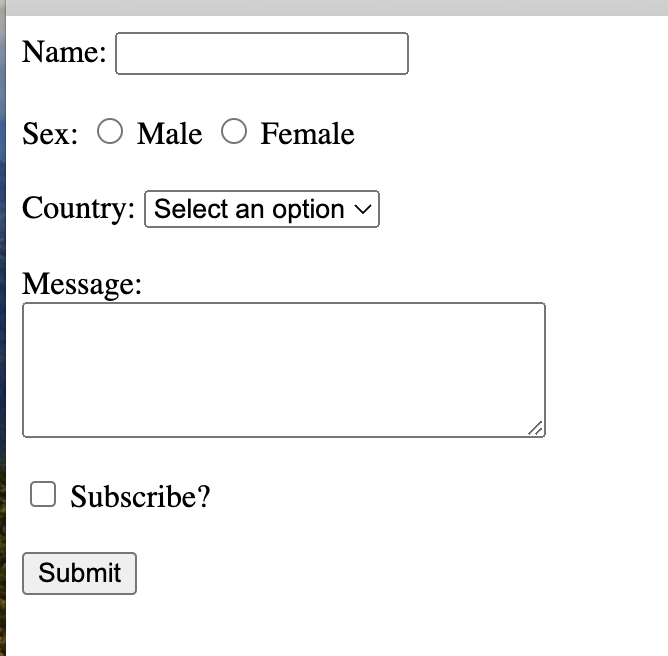
\includegraphics[height=1.7in]{form-1}
        \caption{HTML Form}
        \label{fig:init-form}
    \end{subfigure}%
    ~ 
    \begin{subfigure}[t]{0.5\textwidth}
        \centering
        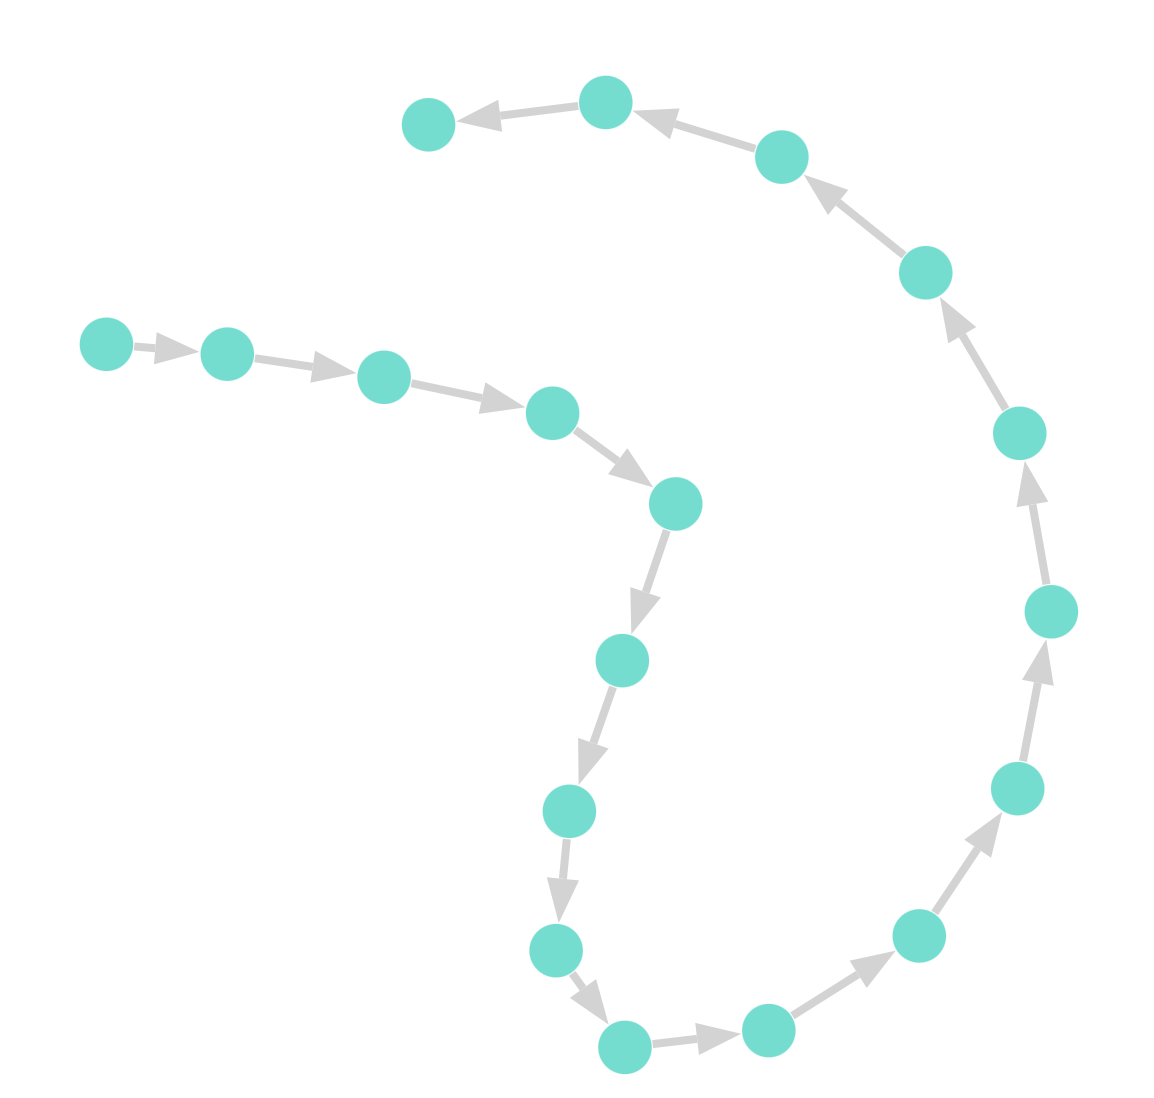
\includegraphics[height=1.7in]{form-1_graph}
        \caption{Graph of Components}
        \label{fig:final-form}
    \end{subfigure}
    \caption{From Form to Graph}
    \label{fig:form-to-graph-eg}
\end{figure*}

The \gls{gnn} consists of several layers, including three convolution layers, a pooling layer, a dropout layer and a dense layer. The task is a binary graph classification task. To generate the features of the dataset, we concatenate the attributes of each vertex and generate word embeddings using GloVe~\cite{pennington-socher-manning:2014}. For each node, we extract the attributes of the node, concatenate them and generate a vector of embeddings of $50$ elements. 

% subsection Web Page Analysis (end)

% section Our Approach (end)
